\section{Tomasz Styn: \texorpdfstring{\\Render Breakdown - od pomysłu do realizacji}{}} % \textorpdfstring pozwala na użycie \\ w nagłówku bez złoszczenia href-a
\label{sec:tstyn}

W tej sekcji przybliżę proces tworzenia animacji w 3D przy pomocy Blendera (\textit{i nie chodzi tu o taki z kuchni!}) Za przykład posłuży mi moja najnowsza praca (patrz: Rysunek~\ref{fig:render_frame})\vspace{2ex} % ref pozwala nam odwołać czytelnika do konkretnej wstaki w naszym dokumencie

\begin{figure}[htbp]
    \centering
    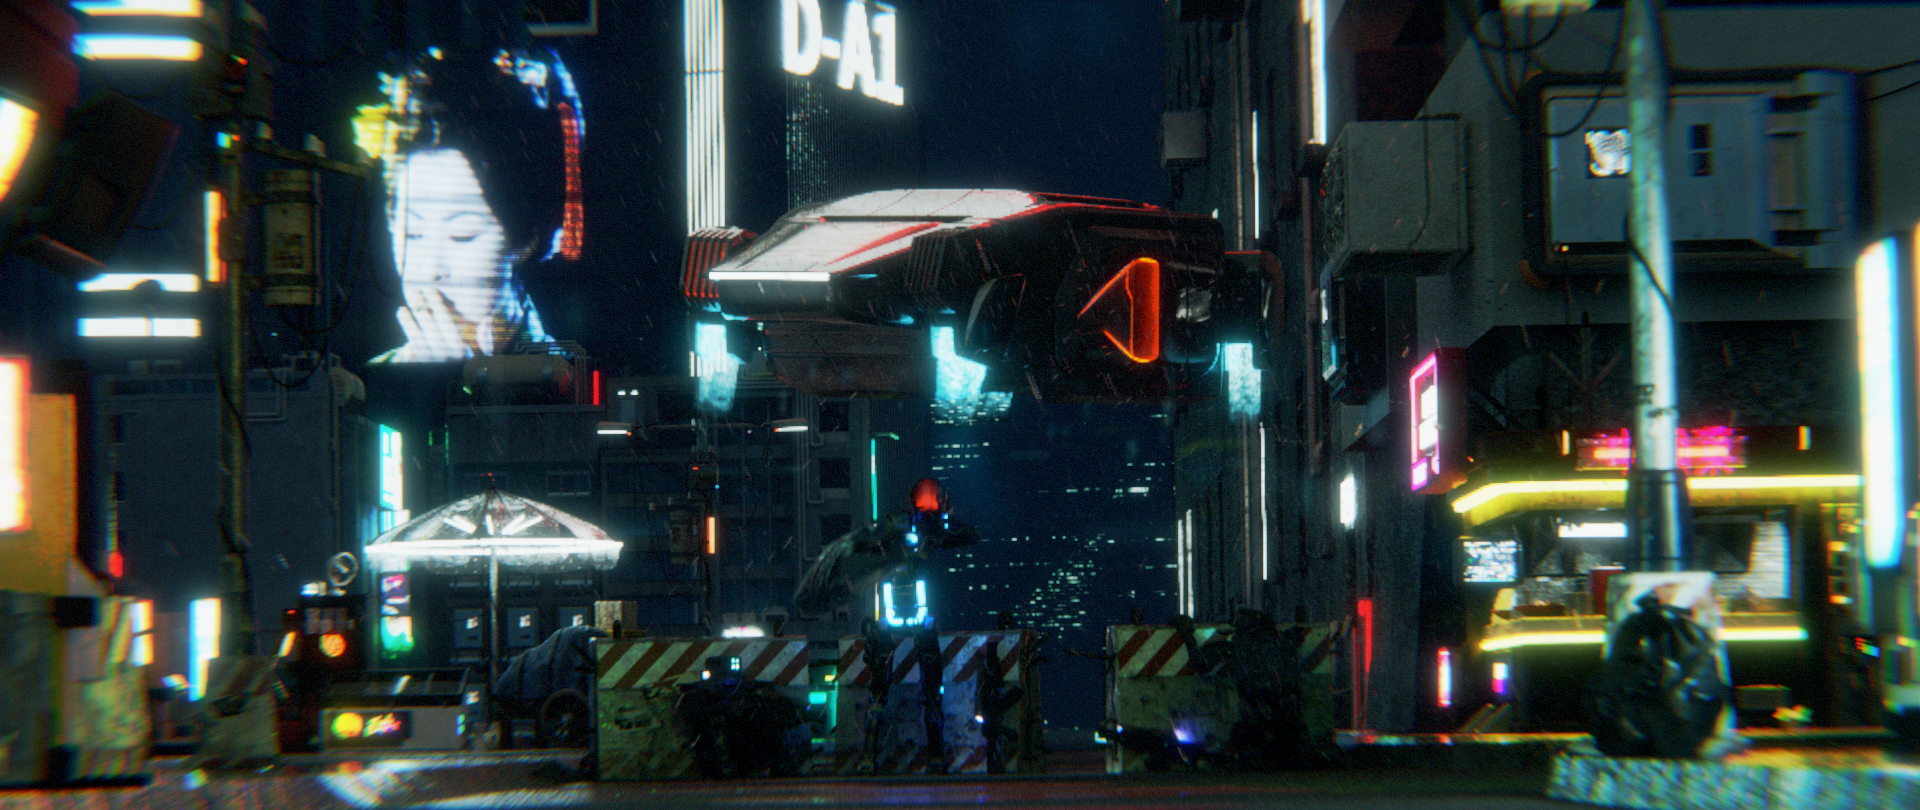
\includegraphics[width=0.95\textwidth]{pictures/Tomek/render_frame.png}
    \caption{Oto 87-ma klatka 5-sekundowej animacji}
    \label{fig:render_frame}
\end{figure}
\vspace{3ex}
W dalszej sekcji przyjrzymy się procesowi tworzenia takiej klatki, wyzwań z tym związanymi oraz zajrzymy za kulisy wykończonej animacji i poznamy kilka sposobów na optymalizację renderowania, które pomogą dotrzymać deadline-ów i oszczędzić na prądzie.

\newpage
\subsection{Jak wpaść na dobry pomysł?}
Jednym z trudniejszych etapów tworzenia rendera od zera jest wpadnięcie na dobry pomysł - wiem, nieco \textit{cliché}, ale tak to wygląda. Jeśli potrzebujesz pomocy z wymyśleniem czegoś ciekawego, polecam przejść przez kilka prostych kroków:
\begin{enumerate}
    \item Poszukaj inspiracji wokół siebie - ludzie, otoczenie, wydarzenia - możesz opisać te rzeczy na własny sposób w swojej pracy
    \item Przejrzyj stare zdjęcia w telefonie - może znajdziesz coś co kiedyś przykuło twoją uwagę, a odtworzenie tego momentu w 3D stanie się dobrym ćwiczeniem i kolejnym punktem w portfolio
    \item Spójrz w głąb samego siebie - szybki rzut oka w mroczną otchłań zagłady prawdopodobnie zaboli, ale też pomoże ją oświetlić; Wyraź to co cię dręczy, cieszy, niepokoi - pokaż światu co ci neurony odbijają od ścian czaszki i zrób to we własnym stylu!
    \item Znajdź interesujący tutorial - nie ma nic lepszego jak poznawanie narzędzia będąc prowadzonym (a czasem ciągniętym) za rękę przez kogoś, kto spędził nad tym co chcesz osiągnąć wiele więcej czasu, niż ciebie na to stać! Potem stwórz analogiczny projekt używając nowo poznanych metod - utrwalisz w ten sposób to, czego się właśnie nauczyłeś i zaadaptujesz do własnych potrzeb - czego chcieć więcej?
    \item Dołącz do wyzwania - coraz częściej artyści z większą społecznością organizują wyzwania renderowe, w których musisz zaadaptować swój pomysł do podanego szablonu oraz elementu przewodniego. Dzięki temu nie musisz zaczynać pomysłu od zera, a do tego możesz coś wygrać! Warto pamiętać, że uczestnictwo w takim wydarzeniu ma na celu pomóc ci poszerzyć swój wachlarz umiejętności - nie chodzi tu o wygraną, a o zgłoszenie pracy z której wykonania sporo się nauczyłeś i jesteś zadowolony z rezultatu!
    \item Zrób rewizję starszego projektu - pamiętasz ren render sprzed półtora roku? Taaaaak, ten którego określenie mianem \textit{spaghetti} gwarantuje ci absolutny, bezwarunkowy zakaz wstępu na teren Włoch - to właśnie on jest idealnym kandydatem na odkupienie swojego wizerunku w oczach mieszkańców gigantycznego półwyspu w kształcie kozaka, których tak bardzo tym podupadłym bałaganem oburzyłeś! Ponowne odwiedzenie starego projektu pokaże Ci jak daleko zaszedłeś, a także da szansę na wykorzystanie nowych technik do poprawienia jego rezultatów!
\end{enumerate}
\newpage
Oczywiście są to tylko wybrane przeze mnie metody, nie krępuj się odtwarzać wymyślonych siedząc do drugiej nad ranem bzdur - one też mają swoją wartość - kto wie, może ty i twoje podtrzymywane przy życiu kofeiną umiejętności modelowania doprowadzą cię na pozycję Picassa grafiki komputerowej! \begin{center}\scriptsize\textit{(UWAGA: Efekt nie jest gwarantowany przez autora pracy! Twoje umiejętności gustownego tworzenia abstrakcji są związane ze stopniem przytomności i obeznaniem z programem 3D. Zapoznaj się z treścią dokumentacji dołączonej do oprogramowania lub skonsultuj się z tutorialem lub forum, gdyż każdy plik nieregularnie zapisywany zagraża utracie lub korupcji godzin roboty.)}\end{center}

\subsection{\texorpdfstring{Okej, mam pomysł i ziemniaczany komputer - \\Co teraz?}{}}
Drogi czytelniku, nadchodzi dobra wiadomość! Na szczęście słaby komputer nie jest ograniczeniem dla twojej kreatywnej ekspresji! Przewagą renderowania pojedynczych kadrów, jak i animacji jest to, że nie musi się ono odbywać in-real-time. Przy pomocy paru sprytnych obejść i standardowych technik z branży VFX nawet dziesięcioletnia, zaklejona na amen sadzą z papierosów i kurzem (na szczęście) nieznanego ci pochodzenia, pożółkła bardziej niż myślałeś że jest to fizycznie możliwe skrzynia twojego dziadka może stać się generatorem najbardziej wyrafinowanych pikseli jakie w życiu widziałeś! \\\textit{(Na dodatek możesz je sobie wypalić na płytce, bo przecież ten relikt ma jeszcze napęd optyczny! Z dyskietkami nawet nie próbuj - potrzebowałbyś pewnie całego dziadkowego archiwum zapyziałych danych na zapis dwóch klatek, nie wspominając o czasie i - na dzisiejsze standardy - zerowej niezawodności zapisu w przypadku użycia tego rozwiązania)}\vspace{1ex} \\ 
Pytasz jakie magiczne sposoby umożliwią ci cyfrową rekreację cudu nad magistralą? Odpowiedzią jest renderowanie w warstwach! Skończyły się dni pochłoniętego teksturami VRAM-u! Absurdalne życzenia klientów zdecydowanie za blisko deadline-u stają się łatwiejsze do wmówienia sobie na siłę ich wykonalności! Myślisz sobie pewnie że to jakaś sztuczka, zamaskowana pod pustymi obietnicami tragicznie skomplikowana technika wymagająca lat doświadczenia - otóż nic bardziej mylnego!\\
Dla użytkowników programów takich jak Photoshop czy Clip Studio Paint, koncepcja warstwy jest dosyć oczywista - dzielimy nasz render na poszczególne składowe klatki. Daje nam to większą kontrolę nad ostatecznym rezultatem, oraz pozwala renderować mniejszą ilość elementów na raz, dzięki czemu redukujemy ilość cache-owanych na raz tekstur i assetów, przyspieszając w ten sposób renderowanie poszczególnych klatek i redukując szanse na crash programu.\newpage
Nauczenie się jak najkorzystniej używać renderowania w warstwach zajmie trochę czasu i eksperymentowania - jest to nieuniknione przy nauce nowych metod zastępujących bardzo podstawowe przyzwyczajenia. Warto jednak poświęcić temu czas - bardziej ambitne projekty w pewnym momencie wymuszą na tobie użycie tego rozwiązania, nie wspominając już o tym, że zmiana jednego elementu scenerii może się skończyć na renderowaniu klatki zawierającej tylko ten element i jego otoczenie zamiast całej sceny od nowa - jedna taka zmiana jest do przeżycia, ale przy większej ich ilości będziesz żałować, że nie podzieliłeś swojej pracy na warstwy. Kolejną zaletą dzielenia klatki na warstwy jest możliwość renderowania różnego stopnia detali dla bardziej i mniej widocznych obiektów - pozwalając nam zaoszczędzić czas podczas renderowania szczegółów, które i tak znajdą się za mgłą, pojawią się na ułamek sekundy, czy zostaną zatarte przez rozmycie przy ruchu kamery. \\
W przykładowej animacji, podzieliłem kadr na 10 warstw, co umożliwiło mi renderowanie tak skomplikowanej sceny. Poniżej (patrz: Tabela~\ref{tab:render-info}) skompilowałem kolejne warstwy, ilość sampli oraz czasy renderowania.

\begin{table}[hbtp]
    \centering
    \caption{Porównanie czasu renderowania poszczególnych warstw}\vspace{0.5ex}
    \begin{tabular}{|| c c c c ||}
        \hline
        Warstwa & Opis & Sample & Czas [mm:ss] \\ [0.5ex]
        \hline\hline
        Mist & Warstwa głębi & 64 & 00:29.17 \\
        \hline
        Rain & Deszcz & 1024 & 00:08.20 \\
        \hline
        FG & Foreground - pierwszy plan & 512 &   00:37.97 \\
        \hline
        AC & Akcja bliżej kamery & 2048 &  01:01.40 \\
        \hline
        Gr & Ground - podłoże & 1024 & 00:46.99 \\
        \hline
        AM & Akcja w środkowym planie & 1024 & 00:27.05 \\
        \hline
        MC & Bliższy midground & 512 & 00:45.43 \\
        \hline
        MF & Dalszy midground & 1024 & 01:19.08 \\
        \hline
        BgC & Tło bliżej & 512 & 00:23.07 \\
        \hline
        BgF & Tło dalej & 256 & 03:11.22 \\ [1ex]
        \hline
    \end{tabular}
    \label{tab:render-info}
\end{table}

Jak widać, w zależności od tego, jak bardzo konkretna warstwa jest skomplikowana i wymagająca, rośnie lub maleje czas potrzebny na jej renderowanie. W podziale na warstwy musimy utrzymać balans między korzyściami z renderowania grup obiektów a ilością warstw\footnote{Dla bardzo uzdolnionych matematycznie czytelników pomocne może być wyrażenie tej zależności za pomocą wzoru: \(t = \frac{complexity}{\# of layers}\), oczywiście w rozsądnych granicach.} - skrajnym przypadkiem byłoby renderowanie każdego assetu osobno, co znacznie spowolniło by proces renderowania oraz zapchało by mnóstwo  miejsca na dysku zapisując głównie puste klatki w wysokiej rozdzielczości w celu późniejszego ich sklejenia. To zagadnienie wprowadza nas w kolejną sekcję.

\newpage
\subsection{Kompozytowanie warstw w gotowe klatki}
Kompozytowaniem nazywamy proces przetwarzania surowych klatek z silnika renderowego w rezultat o pożądanym wyglądzie. W czynności składające się na kompozytowanie możemy zaliczyć na przykład:
\begin{itemize} % Aby zmienić symbol punktowania należy użyć \item[symbol]
    \item Łączenie warstw
    \item Color correction
    \item Nałożenie ziarna
    \item Łączenie renderowanych elementów z materiałem z kamery
    \item Dodanie swojego \textit{czadowego watermarka}
\end{itemize}
Jest to jednak na tyle rozbudowana dziedzina, że istnieją stanowiska pracy i programy takie jak Nuke, które skupiają się jedynie na kompozytowaniu samych renderów jak i łączenia w niezauważalny sposób elementów renderowanych z nagraniem filmowym. W moim projekcie pipeline kompozytora wyglądał następująco:
\begin{figure}[hbtp]
    \centering
    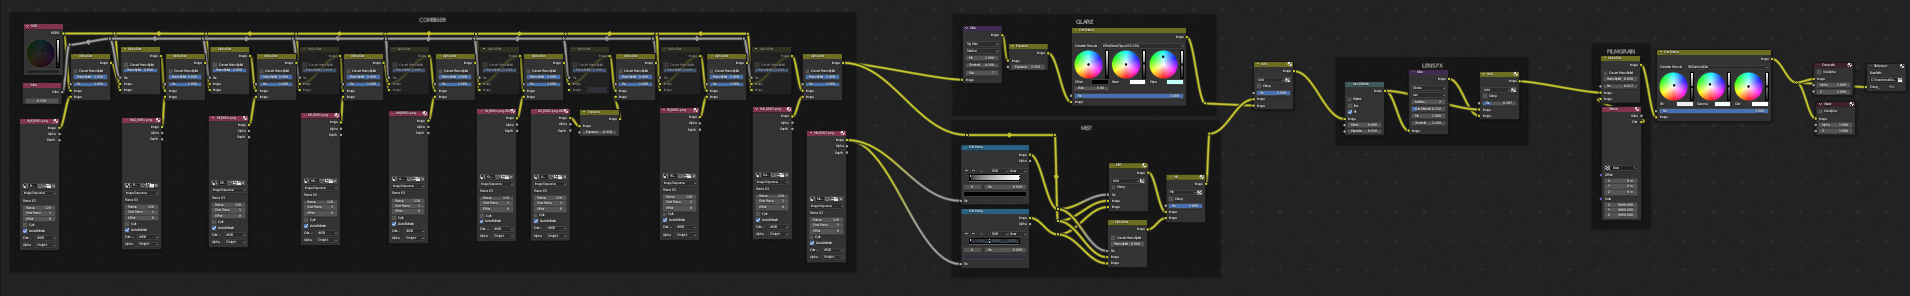
\includegraphics[width=0.95\textwidth]{pictures/Tomek/compositing.png}
    \caption[width=0.75\textwidth]{Tu screenshot pliku który kompozytuje kolejne klatki z osobnych warstw. Następnie przekłada je odpowiednio mgłą o dowolnej przezroczystości, przeprowadza color correction i zapisuje rezultat w odpowiednim pliku. Ten setup jest wystarczająco uniwersalny na potrzeby tego projektu oraz innych o podobnej skali.}
    \label{fig:render_comp}
\end{figure}

Zbliżamy się już do końcowego rezultatu naszej animacji! Zdecydowaliśmy co chcemy przedstwaić w naszej pracy. Dzięki warstwom udało nam się renderować skomplikowaną scenę na słabym sprzęcie i utrzymać naszą pracę w tzw. \textit{industry standard}. Następnie za pomocą podstawowych technik kompozytowania połączyliśmy warstwy zgodnie z naszą wizją, otrzymując w rezultacie setki klatek gotowych do połączenia w animację.
\newpage
\subsection{Łączenie klatek}
Posiadając skompozytowane klatki możemy połączyć je w animację. W tym celu możemy użyć programu takiego jak DaVinci Resolve, albo skorzystać z edytora wideo wbudowanego w Blendera (W Blenderze zrobić można dosłownie wszystko związane z 3D! Do tego- jakimś cudem - jest to darmowy program!). Ja wybrałem drugą opcję ponieważ jestem z nią obeznany.
\begin{figure}[hbtp]
    \centering
    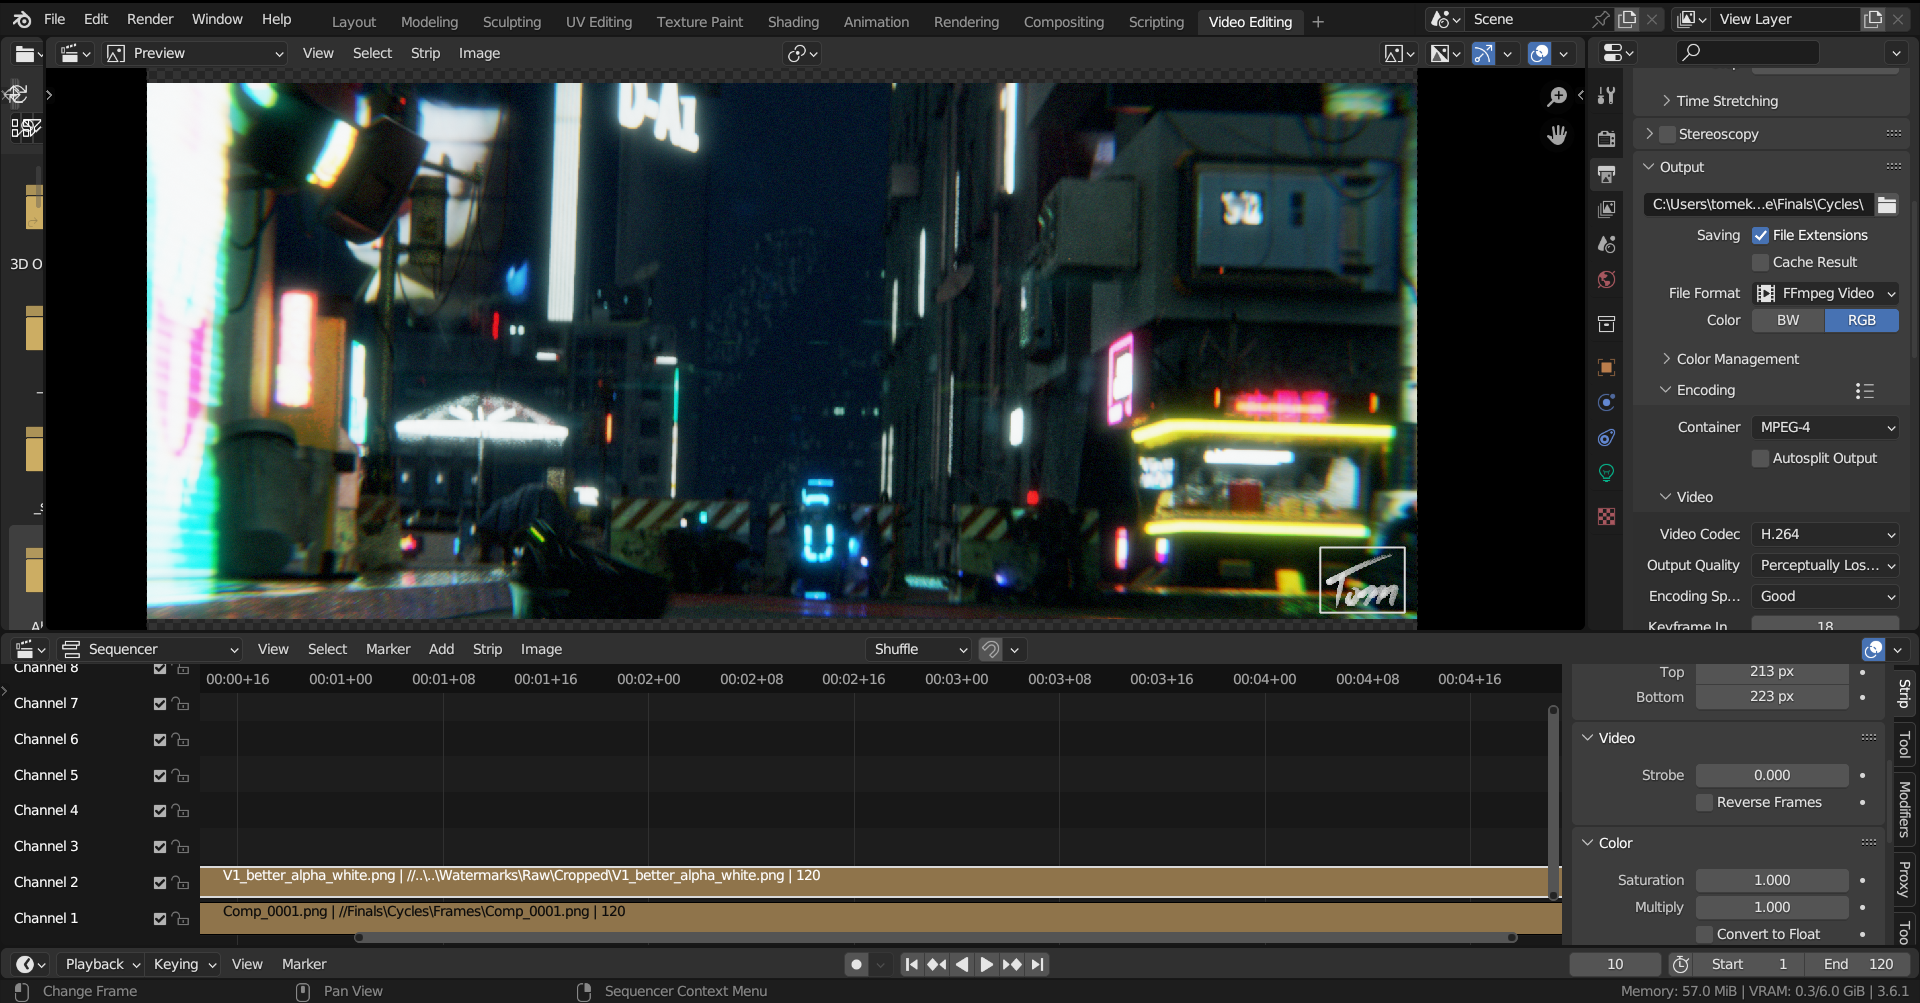
\includegraphics[width=0.9\textwidth]{pictures/Tomek/video_editor.png}
    \caption{Tak wygląda edytor wideo wbudowany w Blendera - na środku widoczny jest podgląd rezultatu, po prawej widzimy opcje encodngu naszej animacji, na dole timeline i kanały zawierające nasze klatki. Kanały w edytorze wideo działają analogicznie do warstw w kompozytorze}
    \label{fig:enter-label}
\end{figure}
\subsection{Podsumowanie}
W ten oto sposób przeszliśmy od pomysłu do gotowej animacji. Czytelniku - mam nadzieję, że udało mi się przybliżyć Ci niektóre aspekty tworzenia pracy w 3D przy pomocy Blendera. Sam ciągle rozwijam swoje umiejętności - części technik, które tu przedstawiłem, nauczyłem się podczas pracy nad projektem który służył nam za przykład. Jeśli masz ochotę obejrzeć tę animację, możesz zrobić to przy pomocy \textcolor{blue}{\href{https://youtu.be/EyG5cc3As4Q}{tego linku}}. \\ % underfull \hbox można zignorować - złości się na to że zostawiłem pustą resztę strony.
\begin{center}
    \textit{Dziękuję za przeczytanie i życzę miłego renderowania!}
\end{center}
\newpage